% !TeX root = ../../Book3.tex
% 纲要标题：### 11.6 Sobolev 延拓与迹
% 纲要位置：几何学计划纲要.md，第 2541 行。
% 正文状态：初稿；尚未正式审核。

% 纲要内容开始
% 
% * 边界展平和延拓算子
% * 迹映射的连续性
% * 零边界 Sobolev 空间
% * 边界正则性的作用
% 
% ---
% 
% 纲要内容结束

\section{Sobolev 延拓与迹}
\label{g3:sec:1106}

给定一个只在区域内部定义的 Sobolev 函数，直接在外部补零通常会在边界产生跳跃。延拓问题问能否用别的方式填补外部，同时控制弱导数；迹问题则问内部的积分控制能否确定一个边界值。两者在半空间中分别归结为反射与一维微积分，光滑边界的作用是把这些局部构造拼到一起。

\subsection{边界展平和延拓算子}
\label{g3:subsec:1106:01}
以下把有界 \(C^1\) 域理解为非空有界开集 \(\Omega\subset\mathbb R^n\)，其边界在每一点附近经刚体运动后是某个 \(C^1\) 函数的图形，且区域位于图形的一侧。结论不要求 \(\Omega\) 连通。\(n=1\) 时，局部模型是区间的端点。先处理
\[
	H=\mathbb R^{n-1}\times(0,\infty),\qquad y=(y',t).
\]

\begin{lemma}\label{g3:lem:half-space-reflection}
	设 \(n\ge1\)、\(1\le p<\infty\)，\(H=\mathbb R^{n-1}\times(0,\infty)\)。对 \(v\in W^{1,p}(H)\)，令
	\[
		(\mathcal Ev)(y',t)=v(y',|t|)\quad(t\ne0).
	\]
	则 \(\mathcal Ev\in W^{1,p}(\mathbb R^n)\)。其切向弱导数为对应导数的偶反射，法向弱导数为 \(\partial_t v\) 的奇反射；函数和梯度的 \(L^p\) 范数均扩大为原来的 \(2^{1/p}\) 倍。
\end{lemma}
\begin{proof}
	关键在于反射后跨过 \(t=0\) 的一维截面没有跳跃。由\cref{g3:prop:weak-line-slices}，对几乎处处的 \(y'\)，函数 \(t\mapsto v(y',t)\) 在 \((0,a)\) 上有绝对连续代表，且函数和导数在此区间可积。其导数的积分在 \(t\downarrow0\) 时收敛，因此该代表有有限端点值，并绝对连续地延伸到 \([0,a]\)。将它偶反射，便得到 \((-a,a)\) 上绝对连续的函数；两侧导数分别为 \(\partial_t v(y',t)\) 和 \(-\partial_t v(y',-t)\)。

	对切向坐标线，在几乎处处的正、负高度处，绝对连续性直接来自原函数的切片。这样，反射函数在每个有界矩形上满足绝对连续切片判据，所列导数就是弱导数。最后分别在 \(t>0\) 与 \(t<0\) 积分、以 \(t\mapsto-t\) 换元，得到范数等式，也得到全空间的可积性。对有限维向量值函数逐分量进行此论证，点态 Euclid 范数和梯度范数仍有同样的反射关系。
\end{proof}

反射后的函数可以在全空间卷积。由\cref{g3:lem:mollifier-approximation}，先在远处截断，再卷积并限制到 \(\overline H\)，得到在边界邻域内也光滑的逼近函数。因此 \(W^{1,p}(H)\) 中的函数可由 \(C_c^\infty(\mathbb R^n)|_{\overline H}\) 逼近；这些逼近函数在 \(t=0\) 上可以非零。

\begin{theorem}\label{g3:thm:sobolev-extension-c1}
	设 \(\Omega\subset\mathbb R^n\) 为有界 \(C^1\) 域，\(1\le p<\infty\)。存在有界线性\term[yantuo suanzi]{延拓算子}[extension operator]
	\[
		E:W^{1,p}(\Omega)\longrightarrow W^{1,p}(\mathbb R^n),
		\qquad Eu|_\Omega=u,
	\]
	以及只依赖 \(\Omega\) 的紧集 \(K\subset\mathbb R^n\)，使
	\[
		\operatorname{supp}Eu\subset K,\qquad
		\|Eu\|_{W^{1,p}(\mathbb R^n)}\le C\|u\|_{W^{1,p}(\Omega)}.
	\]
	常数由维数、\(p\)、有限边界图的尺度及一阶导数界、单位分解的一阶导数界控制。特别地，\(C_c^\infty(\mathbb R^n)|_{\overline\Omega}\) 在 \(W^{1,p}(\Omega)\) 中稠密。
\end{theorem}
\begin{proof}
	在一个边界图中写
	\[
		x_n>f(x'),\qquad
		F(y',t)=(y',t+f(y')).
	\]
	于是 \(F\) 将平边界 \(t=0\) 送到 \(\partial\Omega\)，将 \(t>0\) 送入区域。缩小图的范围后，\(\mathrm DF\)、\(\mathrm DF^{-1}\) 有界，且两者的 Jacobian 行列式为一。\Cref{g3:prop:weak-coordinate-change}给出 \(W^{1,p}\) 范数在此换元下的双向控制。

	取有限个这样的边界图和有限个内部坐标球覆盖 \(\overline\Omega\)，再选光滑单位分解 \(\{\chi_a\}\)，使每个支集紧含于相应的较大图中。对内部项 \(\chi_a u\)，在 \(\Omega\) 外补零即可，因为它已在边界附近消失。对边界项，将 \(\chi_a u\) 拉回半空间。它在图的侧边和上边附近为零，故可在这些人工边界外补零，得到 \(H\) 上的 \(W^{1,p}\) 函数。对它作偶反射，再乘以在其支集上等于一、支集仍留在较大图内的截断函数，最后用 \(F^{-1}\) 送回原坐标。得到的局部延拓在 \(\Omega\) 内恰等于 \(\chi_a u\)。

	将有限个局部延拓相加即定义 \(Eu\)。每一步都是线性的。乘法公式、换元估计与反射引理逐项给出范数界；有限个固定图的闭支集之并给出 \(K\)。在区域内，\(\sum_a\chi_a u=u\)，所以这是所需延拓。

	对 \(Eu\) 在全空间卷积，\(\rho_\varepsilon*Eu\to Eu\) 于 \(W^{1,p}(\mathbb R^n)\)。这些函数光滑且具有紧支集，限制到 \(\Omega\) 便证明最后的稠密性。这里即使边界只有 \(C^1\)，最后的逼近函数也确实是环境空间中的 \(C^\infty\) 函数：光滑化发生在局部构造已经拼成全空间延拓之后。
\end{proof}

\begin{figure}[htbp]
	\centering
	% !TeX root = ../Book3.tex
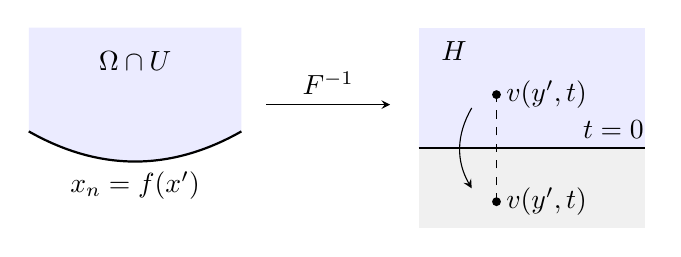
\begin{tikzpicture}[x=.9cm,y=.85cm,>=stealth]
	\fill[blue!8] (0,.25) .. controls (1,-.35) and (2,-.35) .. (3,.25) -- (3,1.8)--(0,1.8)--cycle;
	\draw[thick] (0,.25) .. controls (1,-.35) and (2,-.35) .. (3,.25);
	\node at (1.5,1.3) {\(\Omega\cap U\)};
	\node[below] at (1.5,-.2) {\(x_n=f(x')\)};
	\draw[->] (3.35,.65)--(5.1,.65) node[midway,above] {\(F^{-1}\)};
	\fill[blue!8] (5.5,0) rectangle (8.7,1.8);
	\fill[gray!12] (5.5,-1.2) rectangle (8.7,0);
	\draw[thick] (5.5,0)--(8.7,0);
	\node[above] at (8.25,0) {\(t=0\)};
	\node at (6,1.45) {\(H\)};
	\draw[dashed] (6.6,-.8)--(6.6,.8);
	\fill (6.6,.8) circle (1.6pt) node[right] {\(v(y',t)\)};
	\fill (6.6,-.8) circle (1.6pt) node[right] {\(v(y',t)\)};
	\draw[->] (6.25,.6) to[bend right=30] (6.25,-.6);
\end{tikzpicture}

	\caption[边界展平与反射延拓]{边界展平与反射延拓。左边的图形边界经 \(F^{-1}\) 变为右边的 \(t=0\)；下半空间的值由上半空间对称点的值给定。局部截断使图的侧边不产生新的跳跃。}
	\label{g3:fig:boundary-extension}
\end{figure}

这个定理使有界 \(C^1\) 域满足\cref{g3:def:sobolev-extension-domain}的延拓条件。由\cref{g3:thm:euclidean-sobolev,g3:prop:critical-sobolev,g3:thm:local-morrey}，先对 \(Eu\) 使用全空间估计再限制回来，得到区域上的连续嵌入：当 \(1\le p<n\) 时，\(W^{1,p}(\Omega)\) 嵌入 \(L^{np/(n-p)}(\Omega)\)；当 \(p=n\ge2\) 时，嵌入每个有限 \(L^q\)；当 \(p>n\) 时，有指数 \(1-n/p\) 的连续代表直到边界。\Cref{g3:thm:rellich-domain}同时给出这些嵌入在严格次临界范围内的紧性。一般函数的估计右侧采用完整 \(W^{1,p}\) 范数，因而包含 \(\|u\|_{L^p}\) 项。

\subsection{迹映射的连续性}
\label{g3:subsec:1106:02}
一个 \(L^p(\Omega)\) 等价类可以任意改变边界上的取值，所以不能直接把代表限制到 \(\partial\Omega\)。所需边界值应由内部逼近确定，并且不同逼近必须给出同一结果。一维估计提供了这种唯一性。

\begin{theorem}\label{g3:thm:sobolev-trace}
	设 \(\Omega\subset\mathbb R^n\) 为有界 \(C^1\) 域，\(1\le p<\infty\)，边界测度记为 \(\mathrm dS\)；\(n=1\) 时取端点计数测度。存在唯一有界线性\term[ji yingshe]{迹映射}[trace operator]
	\[
		\operatorname{Tr}:W^{1,p}(\Omega)\longrightarrow L^p(\partial\Omega,\mathrm dS),
	\]
	它在环境光滑函数上等于通常的边界限制。存在 \(h_0>0\) 及 \(C\)，使对 \(0<h<h_0\) 有
	\begin{equation}\label{g3:eq:trace-layer-bound}
		\|\operatorname{Tr}u\|_{L^p(\partial\Omega)}^p
		\le C\left(h^{-1}\|u\|_{L^p(\Omega)}^p
		+h^{p-1}\|\mathrm Du\|_{L^p(\Omega)}^p\right).
	\end{equation}
	若 \(1<p<\infty\)，则对每个 \(\varepsilon>0\)，存在 \(C_\varepsilon\) 使
	\begin{equation}\label{g3:eq:trace-epsilon-bound}
		\|\operatorname{Tr}u\|_{L^p(\partial\Omega)}^p
		\le\varepsilon\|\mathrm Du\|_{L^p(\Omega)}^p
		+C_\varepsilon\|u\|_{L^p(\Omega)}^p.
	\end{equation}
	若 \(u\in W^{1,p}(\Omega)\cap C(\overline\Omega)\)，其迹等于连续代表在边界的值，几乎处处成立。
\end{theorem}
\begin{proof}
	先对平半柱中的光滑函数 \(v(y',t)\) 使用微积分基本公式。对 \(0<t<h\)，有
	\[
		|v(y',0)|^p
		\le2^{p-1}|v(y',t)|^p
		+2^{p-1}t^{p-1}\int_0^t|\partial_t v(y',s)|^p\,\mathrm ds.
	\]
	这里 \(p=1\) 直接用积分三角不等式，其余情形用 Hölder 不等式。对 \(t\in(0,h)\) 取平均，再对 \(y'\) 积分，得到
	\[
		\int|v(y',0)|^p\,\mathrm dy'
		\le2^{p-1}\left(h^{-1}\int_0^h\!\int|v|^p\,\mathrm dy'\mathrm dt
		+h^{p-1}\int_0^h\!\int|\partial_t v|^p\,\mathrm dy'\mathrm dt\right).
	\]
	在每个边界图中令 \(v=(\chi_a u)\circ F\)。表面积元是 \(\sqrt{1+|\mathrm Df|^2}\,\mathrm dy'\)，它与 \(\mathrm dy'\) 一致可比。换元和乘法估计把右侧变成 \(u\) 与 \(\mathrm Du\) 的积分；由 \(\mathrm D\chi_a\) 产生的 \(h^{p-1}\|u\|_p^p\) 项在 \(h<h_0\le1\) 时并入 \(h^{-1}\|u\|_p^p\)。有限求和即得式\eqref{g3:eq:trace-layer-bound}。

	固定一个允许的 \(h\)，便得光滑函数的有界迹估计。由\cref{g3:thm:sobolev-extension-c1}的稠密性，若 \(u_j\to u\) 于 \(W^{1,p}\)，则边界限制 \(u_j|_{\partial\Omega}\) 是 \(L^p(\partial\Omega)\) 中的 Cauchy 列。定义其极限为 \(\operatorname{Tr}u\)。同一估计应用于两个逼近序列之差，证明定义无关；它也证明线性、有界性及唯一性，并使薄层估计延续到全部 \(u\)。当 \(p>1\) 时，选 \(h\) 使 \(Ch^{p-1}\le\varepsilon\)，即得式\eqref{g3:eq:trace-epsilon-bound}。

	若 \(u\) 在闭包连续，前一定理中的反射、截断和有限求和给出一个连续紧支延拓。它的卷积同时在闭包上一致收敛到 \(u\)，又在 \(W^{1,p}\) 中收敛。因此其边界限制的 \(L^p\) 极限就是 \(u|_{\partial\Omega}\)，证明最后一项。
\end{proof}
\symidx{\(\operatorname{Tr}u\)：Sobolev 函数或截面的边界迹}

薄层估计还显示了尺度。对一个固定的 \(C^1\) 域 \(\Omega_1\) 及 \(\Omega_R=R\Omega_1\)，换元 \(x=Ry\) 给出
\[
	\|\operatorname{Tr}u\|_{L^p(\partial\Omega_R)}^p
	\le C\left(R^{-1}\|u\|_{L^p(\Omega_R)}^p
	+R^{p-1}\|\mathrm Du\|_{L^p(\Omega_R)}^p\right).
\]
左侧在缩放中有 \(n-1\) 维的因子，两个右侧项恰有相同尺度。

\ProseParagraphBreak

\(p=1\) 时，式\eqref{g3:eq:trace-layer-bound}仍成立，但梯度前的系数不随 \(h\downarrow0\) 消失。例如在一个平边界片取非零光滑紧支 \(\psi(y')\)，再取 \(\eta(0)=1\)、支集位于 \([0,1)\) 的光滑函数，令 \(v_\delta(y',t)=\psi(y')\eta(t/\delta)\)。它的内部 \(L^1\) 范数趋零，\(\|\mathrm Dv_\delta\|_{L^1}\) 保持有界，而边界迹恒为 \(\psi\)。选足够小的固定 \(\varepsilon\) 就能看出，一般不能把式\eqref{g3:eq:trace-epsilon-bound}中的任意小系数结论扩展到 \(p=1\)。

\begin{proposition}\label{g3:prop:weak-boundary-integration}
	设 \(\Omega\subset\mathbb R^n\) 为有界 \(C^1\) 域，\(1\le p<\infty\)，\(u\in W^{1,p}(\Omega)\)，\(\phi\) 在 \(\overline\Omega\) 的邻域中光滑。若 \(\nu\) 为外单位法向，则
	\begin{equation}\label{g3:eq:weak-boundary-integration}
		\int_\Omega u\,\partial_i\phi\,\mathrm dx
		=-\int_\Omega(\partial_i u)\phi\,\mathrm dx
		+\int_{\partial\Omega}(\operatorname{Tr}u)\phi\nu_i\,\mathrm dS.
	\end{equation}
\end{proposition}
\begin{proof}
	先取光滑 \(u\)。在图形区域 \(x_n>f(x')\) 内，沿 \(x_n\) 积分给出下端点项；切向积分时，对变动下限 \(f(x')\) 求导，给出 \(\partial_i f\) 的因子。这恰是
	\[
		\nu\,\mathrm dS=(\mathrm Df,-1)\,\mathrm dx'
	\]
	的各分量。用单位分解求和，内部片无边界项，单位分解的导数因其总和为一而相消，得到光滑函数的公式。最后用贴边光滑函数在 \(W^{1,p}\) 中逼近 \(u\)。区域和边界测度都有限，内部两项按 \(L^p\) 收敛，边界项按迹的连续性收敛，故公式成立。
\end{proof}

\subsection{零边界 Sobolev 空间}
\label{g3:subsec:1106:03}
\(W_0^{1,p}(\Omega)\) 按定义是 \(C_c^\infty(\Omega)\) 的 \(W^{1,p}\) 闭包。它首先描述可逼近性。下面证明，在规则边界上，这个闭包恰好实现零边界值；零延拓是否产生额外边界导数是两种描述之间的联系。

\begin{theorem}\label{g3:thm:zero-trace-characterization}
	设 \(\Omega\subset\mathbb R^n\) 为有界 \(C^1\) 域，\(1\le p<\infty\)，\(u\in W^{1,p}(\Omega)\)。记 \(\widetilde u\) 为 \(u\) 在 \(\mathbb R^n\setminus\Omega\) 上补零的函数。则以下条件等价：
	\begin{equivalences}
		\item \(u\in W_0^{1,p}(\Omega)\)；
		\item \(\operatorname{Tr}u=0\)；
		\item \(\widetilde u\in W^{1,p}(\mathbb R^n)\)。
	\end{equivalences}
	此时 \(\partial_i\widetilde u=\widetilde{\partial_i u}\)，几乎处处成立。
\end{theorem}
\begin{proof}
	若 \(u\in W_0^{1,p}\)，用紧支于 \(\Omega\) 的光滑函数逼近。它们的迹都是零，故由连续性得到第二项；它们的零延拓及其导数在全空间同样是 Cauchy 列，故也得到第三项及所列导数公式。

	若 \(\operatorname{Tr}u=0\)，对任意 \(\phi\in C_c^\infty(\mathbb R^n)\)，式\eqref{g3:eq:weak-boundary-integration}成为
	\[
		\int_{\mathbb R^n}\widetilde u\,\partial_i\phi\,\mathrm dx
		=-\int_{\mathbb R^n}\widetilde{\partial_i u}\,\phi\,\mathrm dx.
	\]
	右侧由一个 \(L^p\) 函数给出，所以零延拓属于 \(W^{1,p}\)，并具有指定弱导数。

	现在从第三项构造内部紧支逼近。这一步既适用于 \(p>1\)，也适用于 \(p=1\)。用前述有限单位分解将 \(u\) 分成内部项与边界项。内部项离边界有正距离，直接卷积即可。对边界项，将其零延拓通过展平坐标拉回，得到一个紧支 \(w\in W^{1,p}(\mathbb R^n)\)，且 \(w=0\) 于 \(t<0\)。令
	\[
		w_\delta(y',t)=w(y',t-\delta),\qquad \delta>0.
	\]
	这将支集向区域内部移动，因而 \(w_\delta=0\) 于 \(t<\delta\)。由 \(L^p\) 平移连续性，函数及其全部一阶弱导数都收敛，所以 \(w_\delta\to w\) 于 \(W^{1,p}\)。再取卷积半径 \(\varepsilon_\delta<\delta/2\)，使卷积误差趋零。所得光滑函数的支集仍在 \(t>\delta/2\)，并可使其始终留在原来较大的坐标图内。

	将这些函数送回原坐标，得到离 \(\partial\Omega\) 有正距离的紧支 \(C^1\) 函数。若边界图只有 \(C^1\)，再对每个这样的函数在原 Euclid 坐标中作一次足够小半径的卷积，便得到 \(C_c^\infty(\Omega)\) 函数，且误差可任意小。换元估计保证此前的收敛仍为 \(W^{1,p}\) 收敛。有限个局部项相加，就得到逼近 \(u\) 的内部紧支光滑序列，证明第一项。
\end{proof}

例如区间上的常函数一属于 \(W^{1,p}(0,1)\)，但不属于 \(W_0^{1,p}(0,1)\)。它的零延拓是区间的示性函数，分布导数为 \(\delta_0-\delta_1\)，并非 \(L^p\) 函数。边界跳跃恰对应刚才分部积分中没有消失的边界项。

\ProseParagraphBreak

对非零给定边界数据，若已选定一个提升 \(g\in W^{1,p}(\Omega)\)，则所有满足 \(\operatorname{Tr}u=\operatorname{Tr}g\) 的函数恰为
\[
	g+W_0^{1,p}(\Omega).
\]
这是迹的线性与核的刻画直接给出的仿射空间。以后构造弱解时，减去 \(g\) 就把边界条件化为零边界条件。

\subsection{边界正则性的作用}
\label{g3:subsec:1106:04}
前面的常数来自有限个图的大小、展平映射及逆映射的导数、表面积元与单位分解。对一族区域，如果这些量一致受控，构造就给出一致的延拓与迹估计。仅知道各个区域分别有光滑边界，并不能使这些常数自动一致。

\begin{proposition}\label{g3:prop:sobolev-boundary-bundles}
	设 \((M,g)\) 为紧的光滑 \(n\) 维带边界黎曼流形，\(E\to M\) 为带光滑纤维度量及相容联络的有限秩实或复向量丛，\(1\le p<\infty\)。则存在有界线性映射
	\[
		\operatorname{Tr}:W^{1,p}(M;E)\longrightarrow
		L^p(\partial M;E|_{\partial M}),
	\]
	它延拓光滑截面的边界限制，且
	\[
		\ker\operatorname{Tr}=W_0^{1,p}(M;E),
	\]
	右侧为内部紧支光滑截面的闭包。式\eqref{g3:eq:trace-layer-bound}和 \(p>1\) 时的式\eqref{g3:eq:trace-epsilon-bound}也成立，将 \(\mathrm D\) 换为 \(\nabla\)、体积及表面积换为诱导的密度即可。相应的一阶嵌入范围为：
	\begin{enumerate}
		\item 当 \(1\le p<n\) 时，连续嵌入 \(L^q(M;E)\)，\(1\le q\le np/(n-p)\)；严格小于该上端点时嵌入为紧。
		\item 当 \(p=n\ge2\) 时，对每个 \(1\le q<\infty\)，到 \(L^q(M;E)\) 的嵌入为紧，因而连续。
		\item 当 \(p>n\) 时，连续嵌入 \(C^{0,\alpha}(M;E)\)，\(\alpha=1-n/p\)；到 \(C^{0,\beta}(M;E)\) 的嵌入在 \(0\le\beta<\alpha\) 时为紧，这里 \(\beta=0\) 表示一致范数。
		\item 当 \(n=p=1\) 时，连续嵌入 \(C^0(M;E)\)，并紧嵌入每个有限 \(L^q(M;E)\)。
	\end{enumerate}
	Hölder 范数按有限坐标图与丛标架定义。
\end{proposition}
\begin{proof}
	取有限个内部图及边界半空间图，并在各图内选择光滑丛标架。将截面乘以单位分解后逐分量反射、卷积，得到直到边界都光滑的逼近截面。局部范数与 \(\sum(|u^a|^p+|\mathrm Du^a|^p)\) 的积分等价：体积密度和纤维度量有正的上下界，协变导数与普通导数相差有界联络系数乘以截面的零阶项。

	各分量的边界迹因而满足一致的有限图估计。在两组标架的交集，分量由一个光滑可逆矩阵联系；在光滑截面上，取边界值与该矩阵的限制相容。再用逼近与乘法连续性取极限，这个相容关系保留，所以局部迹粘成 \(E|_{\partial M}\) 的截面，与标架及单位分解无关。标量证明中的分部积分、零延拓和向内平移逐分量进行，证明核正是内部紧支光滑截面的闭包。

	对每个局部项用半空间延拓，再使用欧氏 Sobolev 与 Rellich 结论，便得到相应的连续嵌入与紧嵌入；紧性只需对有限个图依次取子列。范数等价负责把分量收敛还原成截面收敛。迹的薄层估计也逐图求和；联络及截断引入的零阶项并入已有零阶项，便得到所述两种估计。
\end{proof}

\begin{proposition}\label{g3:prop:higher-order-boundary-extension}
	设 \(k\ge1\) 为整数，\(\Omega\subset\mathbb R^n\) 是有界 \(C^k\) 域，\(1\le p<\infty\)。则存在有界线性延拓
	\[
		E_k:W^{k,p}(\Omega)\longrightarrow W^{k,p}(\mathbb R^n),
	\]
	其支集包含于一个固定紧集。该构造的常数由有限边界图及逆图直到 \(k\) 阶的导数和相应截断函数控制。
\end{proposition}
\begin{proof}
	半空间上的偶反射一般不能保留二阶弱导数，例如 \(v(t)=t\) 的偶反射为 \(|t|\)，其一阶导数在零处跳跃。为使直到 \(k-1\) 阶的法向导数匹配，选择 \(c_1,\ldots,c_k\) 满足
	\[
		\sum_{j=1}^k c_j(-j)^\ell=1,
		\qquad 0\le\ell\le k-1.
	\]
	这些系数存在且唯一：系数矩阵可逆，因为次数不超过 \(k-1\) 的多项式若在 \(-1,\ldots,-k\) 都为零，就恒为零。对在闭半空间光滑的 \(v\)，在 \(t<0\) 定义
	\[
		(E_kv)(y',t)=\sum_{j=1}^k c_jv(y',-jt),
	\]
	在 \(t\ge0\) 保留原值。上述等式使所有总阶数小于 \(k\) 的导数在两侧相接。逐次分部积分时，直到第 \(k\) 次求导都没有边界跳跃项。每项的 \(\ell\) 次法向导数只多出 \((-j)^\ell\)，再以 \(s=-jt\) 换元，便得到 \(W^{k,p}\) 范数界。

	这里所用的闭半空间光滑稠密性也可在任意整数阶直接建立。先在远处截断，随后将 \(v(y',t)\) 替换为 \(v(y',t+\delta)\)。后者在 \(t>-\delta\) 已有定义；其各阶弱导数在 \(H\) 上趋于原导数，这是将这些 \(L^p(H)\) 导数各自补零后应用平移连续性的结果。再在半径小于 \(\delta/2\) 内卷积，得到闭半空间附近光滑的函数；对所有不超过 \(k\) 阶的导数同时选择足够小的卷积半径，就得到 \(W^{k,p}(H)\) 逼近。因此前述有界反射算子可连续延拓到全部 \(W^{k,p}(H)\)。

	对一般 \(C^k\) 域，使用与一阶情形相同的有限覆盖、单位分解及展平。反复使用链式法则，\(C^k\) 图及逆图的有界导数控制全部不超过 \(k\) 阶的范数。将半空间延拓限制在足够薄的较大图内、乘截断后送回并求和，就得到所需算子与固定紧支集。
\end{proof}

这个证明说明了所选展平构造为何要求相应阶数的导数控制。\(C^1\) 边界也不是一阶延拓存在的必要条件：矩形的角点不满足 \(C^1\) 图形条件，但逐个坐标反射、再乘固定截断函数，仍给出一阶有界延拓。判断边界正则性时，要检查实际能否作有界的局部变换与拼接。

\begin{example}\label{g3:exm:slit-domain-traces}
	考虑去掉一条半径的单位圆盘
	\[
		\Omega=\{(r\cos\theta,r\sin\theta):0<r<1,\ 0<\theta<2\pi\}.
	\]
	取 \(\chi\in C_c^\infty((1/4,3/4))\)，且在一个较小区间上等于一，定义 \(u(r,\theta)=\chi(r)\theta\)。函数及其一阶导数在 \(\Omega\) 上有界，所以 \(u\in W^{1,p}(\Omega)\) 对每个有限 \(p\) 成立。裂缝的上侧边界值为零，下侧为 \(2\pi\chi(r)\)，两侧都来自各自半邻域中的光滑限制。

	不存在把这个 \(u\) 延拓到整个圆盘的 \(W^{1,p}\) 函数。事实上，对裂缝中 \(\chi=1\) 的一段，几乎每条横穿裂缝的竖直线在两侧都有相差 \(2\pi\) 的极限。若延拓属于 \(W^{1,p}\)，绝对连续切片判据要求同一条线上的代表跨过裂缝连续，矛盾。裂缝作为平面中的点集只有一份，但域内逼近有两侧；在这种区域上，边界值必须保留所从属的一侧。
\end{example}
% 纲要条目排为编号小节标题，并进入目录与书签；说明段仍保留于纲要注释中。
